\documentclass{beamer}

\usepackage{hyperref}

\usetheme{Antibes}

\title{Maintainable Embedded Linux Solutions}
\author{Thomas Irgang \and Simone Weiß}
\institute{EASTERHEGG 2024 - RABBIT PROTOTYPING}
\date{March 31, 2024}
\titlegraphic{
    
\includegraphics[width=2cm]{assets/logo.png}
}

\newcommand\pro{\item[$+$]}
\newcommand\con{\item[$-$]}

\begin{document}

\begin{frame}
    \titlepage
\end{frame}

\begin{frame}
	\begin{block}{Topic}
		How to build long-term secure and maintainable embedded Linux solutions
		while spending limited effort to keep the solution secure?
	\end{block}
	% Hi ...
	% We spend lot's of time to build feature-rich embedded systems with a lifetime of
	% 15 years and more. Nowadays, these systems are Linux based and connected to the
	% internet, which makes security an important topic.
	% In this talk, we want to share with you our insides and ideas how to build
	% embedded systems with a lifetime more than 15 years which don't require
	% tousands of hours each year to keep them secure.
\end{frame}

\section{Is Linux the right choice?}

\begin{frame}{Do I need Linux for my project?}
	Before we begin:

	\begin{block}{Rule}
		Smaller is better!
	\end{block}
	
	\begin{itemize}
		\item Less interfaces means less attack surface!
		\item Less software means less maintenance effort!
	\end{itemize}
	% A first learning we have made is: "Smaller is better".
	% If the solution has less interfaces, the attack surface is much smaller,
	% and less software means less CVEs to care about, and less unkown bugs and
	% security issues.
	% This is true with respect to embedded Linux, but also true when you select
	% the hardware for your project.
\end{frame}

\begin{frame}{Do I need Linux for my project?}
	\begin{tabular}{cccc}
	&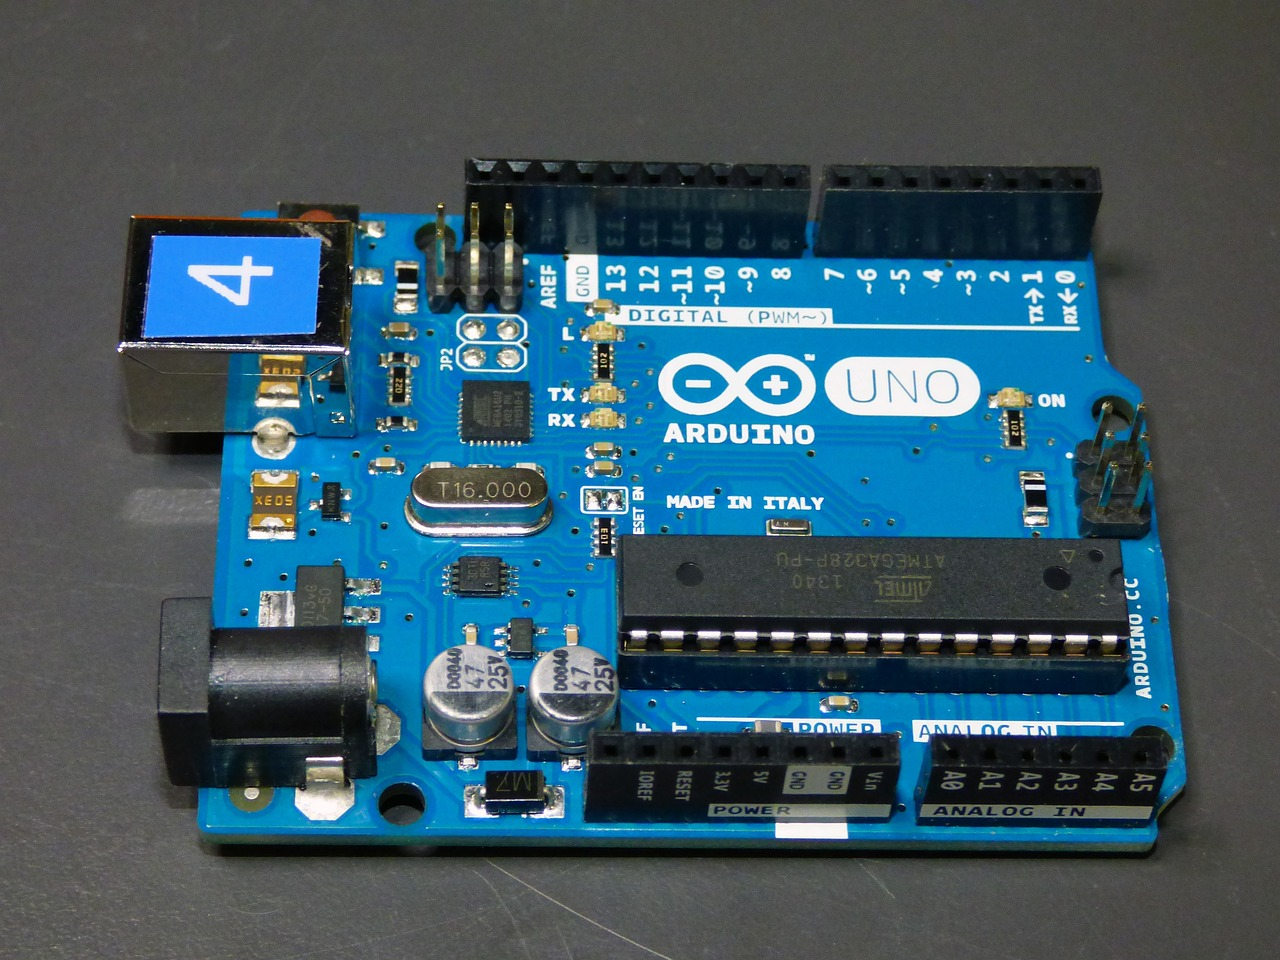
\includegraphics[width=1.9cm]{assets/Pixabay_Arduino_integrated-circuit-441289_1280.jpg} &
	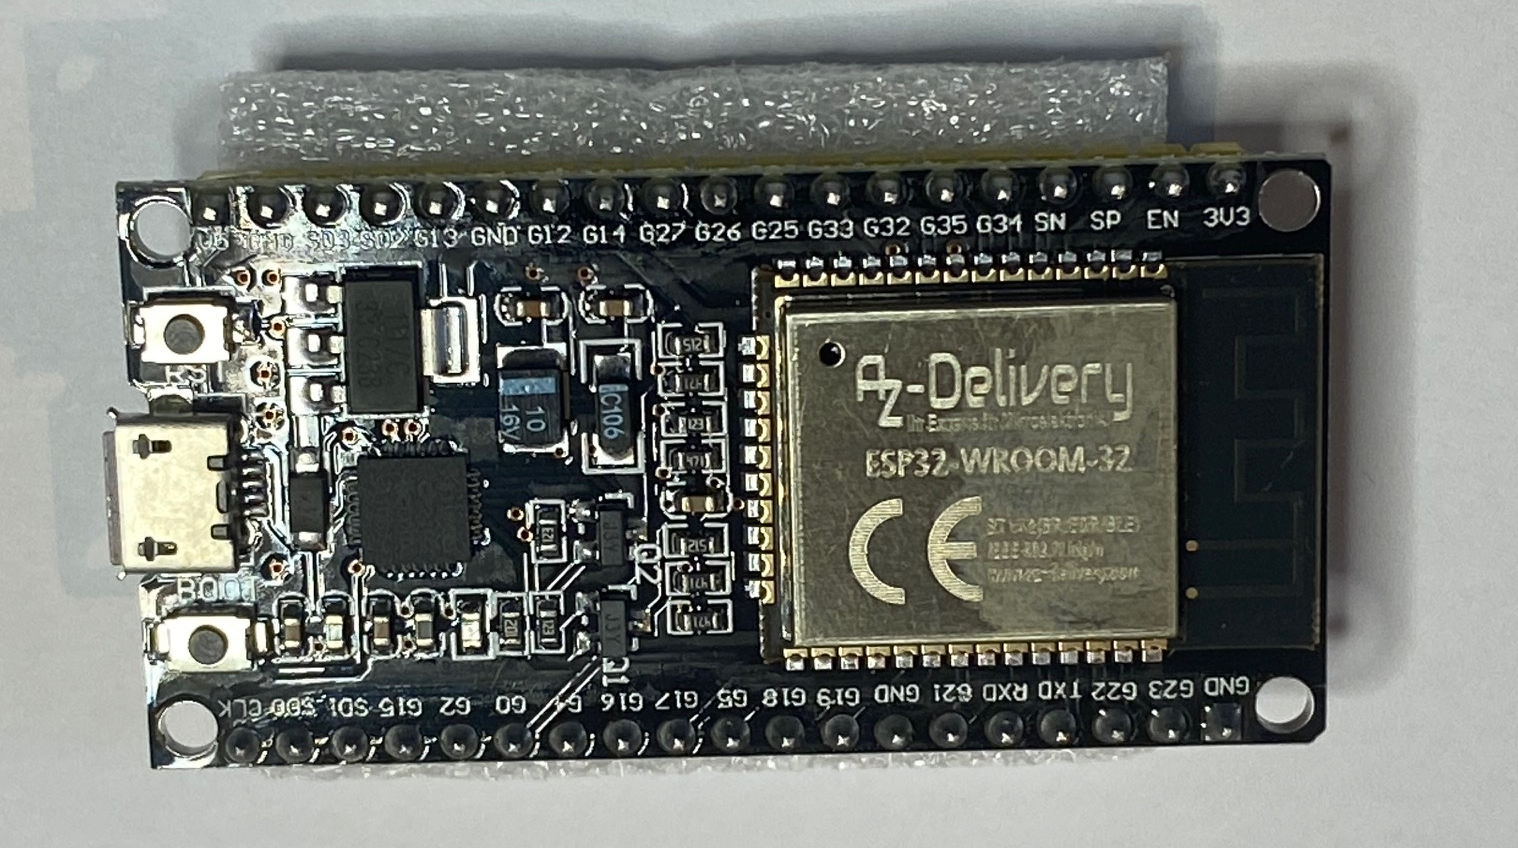
\includegraphics[width=1.9cm]{assets/ESP32.png} & 
	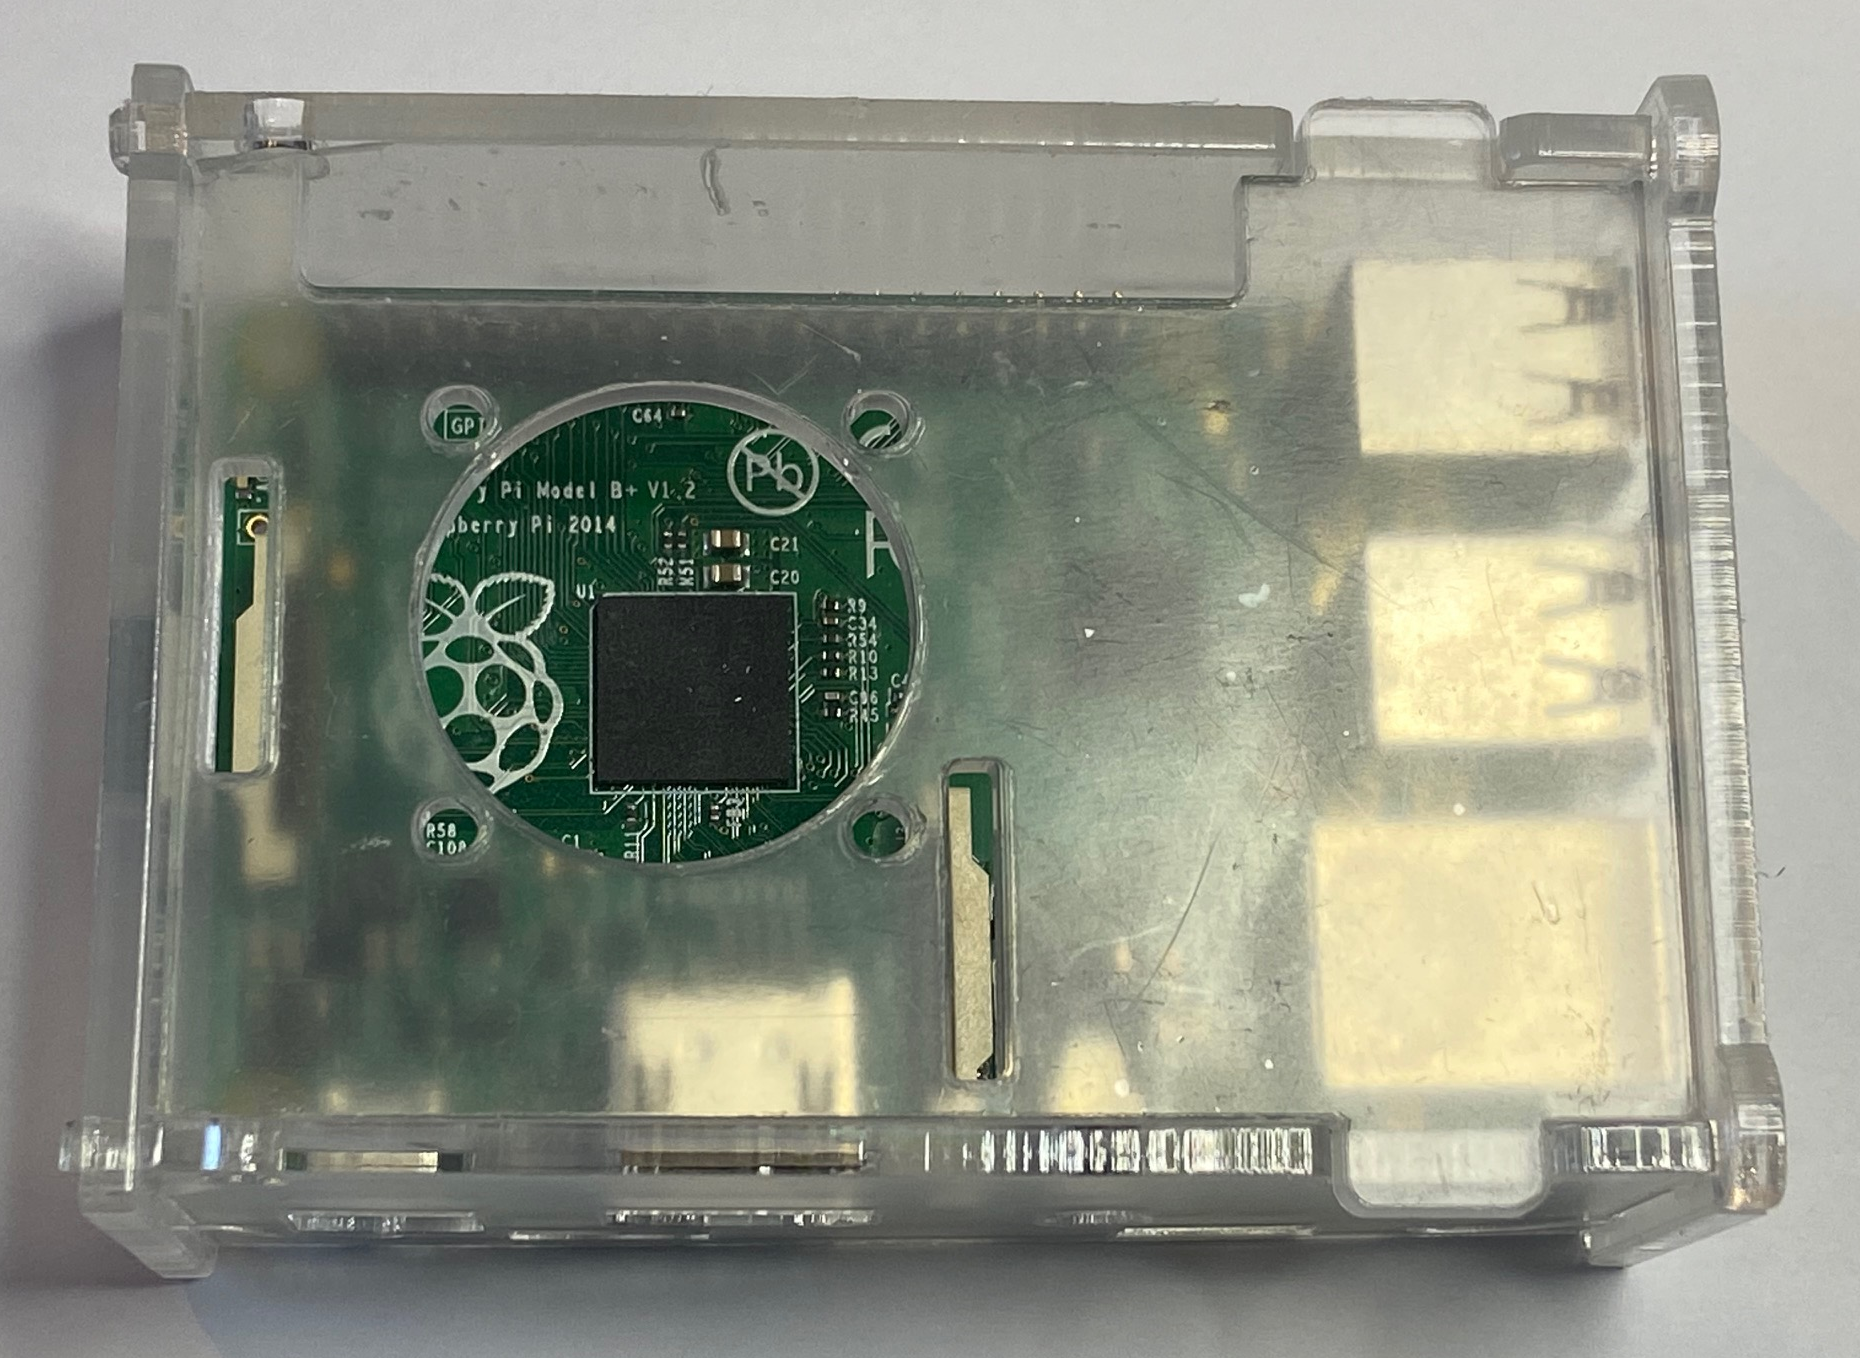
\includegraphics[width=1.9cm]{assets/Raspberry_Pi.png} \\
	&\textbf{Arduino} & \textbf{ESP32 FreeRTOS} & \textbf{SBC Linux} \\
	real-time & + &  + & - \\
	energy & + & o & - \\
	communication & - & o & + \\
	\end{tabular}
	% If you choose the right hardware platfrom for your problem, you can
	% save a lot of development effort and later maintenance effort.
	% If you want to build a small sensor or control unit with real time needs,
	% an Arduino may be a way better choice than a Raspberry Pi, and if you
	% don't need WiFi, don't use it. This reduces the attack surface a lot.
	% If you want to build a small IoT device, an ESP32 and FreeRTOS may be 
	% a way better choice than an SBC running Linux.
	% This security considerations also hold true with respect to energy
	% consumption and other environmental concerns.
	% If your embedded system requires a lot of  communication and maybe
	% also a rich UI, a SBC and Linux may be a good choice.
\end{frame}

\begin{frame}{What's the life-time of my project?}
	\begin{block}{What's the life-time?}
		Do I need to care about maintenance and updates?
	\end{block}
\end{frame}

\begin{frame}{What's the life-time of my project?}
	\begin{columns}[t]
    \column{0.33\textwidth}
        \centering
        \textbf{Experiment}
        \begin{itemize}
        		\item few months
        		\item no maintenance
        		\item some reusability
        \end{itemize}
    \column{0.33\textwidth}
        \centering
        \textbf{Media-Center}
        \begin{itemize}
        		\item some years
        		\item typical IT distribution maintenance
        		\item no reusability needed
        \end{itemize}
    \column{0.34\textwidth}
        \centering
        \textbf{Home Automation}
        \begin{itemize}
        		\item more than 15 years
        		\item \emph{maintenance and upgrades}
        		\item \emph{reusability for mid-term upgrade needed}
        \end{itemize}
    \end{columns}
	% The next aspect you should consider in the very beginning of your
	% project is the nature and lifetime of the project.
	% If your goal is to learn or prototype something, and running the
	% result is not in your interest, then maintenance or energy considerations
	% may be not relevant. But be careful: Nothing lasts as long as a temporary
	% solution.
	% If you want to build some project with expected limited lifetime, like a
	% mediacenter where you will update after some years to get the latest
	% software and hardware accelerator support, then a typical IT Linux 
	% maintenance may be ok, and maintenance is a quite small problem.
	% If you want to build long living solutions, like your hackspace automation,
	% your mat-o-mat or your coffee machine, you should consider the maintenance
	% and resource consumption from the beginning. 
\end{frame}

\section{Embedded Linux}

\begin{frame}{How to build an embedded Linux distribution?}
	\begin{block}{Topic}
		How to build a project specific embedded Linux distribution?
	\end{block}
	% Let's assume you came to the conclusion that embedded Linux is the 
	% best choice for your project.
	% Then, the next question is how to build the embedded Linux image for
	% the SD card or eMMC.
	% We are aware of three different approaches to build embedded Linux
	% images and will give you a short overview.
\end{frame}

\begin{frame}{The "golden image" approach}
	\begin{itemize}
		\item starting from an existing Linux image, e.g. Raspberry Pi OS,
		\item install the required tools,
		\item and configure it,
		\item and freeze the image.
	\end{itemize}

	\begin{columns}[t]
    \column{0.5\textwidth}
        \centering
        \begin{itemize}
			\pro easy approach
			\pro maintained by used distribution
		\end{itemize}        
    \column{0.5\textwidth}
        \centering
        \begin{itemize}
        		\con solution and base distribution are mixed
        		\con no support for variants
        		\con lots of not needed software
        \end{itemize}
    \end{columns}
	% The approach you most likely all know is what we call the "golden image"
	% approach. You take an existing Linux image for your SBC, for example
	% Raspberry Pi OS, install the packages you need and configure the image.
	% When you think it's ready, you do a snapshot.
	% This is for sure the most easy approach, and for the first years
	% your maintenance is running apt update and apt upgrade.
	% The challenges start when you want to run this system longer than
	% the used distribuiton is supported, or when the updates break
	% your project and you need to remember what you have done and
	% configured a few years ago.
	% It also gets complicated when you want to have variants of the solution,
	% because then you need to keep your images manually in sync for all
	% common features.
	% This approach also has the drawback that you have lots of software 
	% and running services you don't need, but these services may have
	% security issues and also increase the energy consumption and hardware
	% needs of your project. 
\end{frame}

\begin{frame}{The "from scratch" approach}
	\begin{itemize}
		\item using a built toolkit, e.g. Yocto or Buildroot
		\item which builds all packages from source
		\item using a project specific configuration and patches
	\end{itemize}

	\begin{columns}[t]
    \column{0.5\textwidth}
        \centering
        \begin{itemize}
        	\pro optimal system
        	\pro minimized resources
        	\pro reusable solution
        	\pro support for variants
        \end{itemize}
    \column{0.5\textwidth}
        \centering
        \begin{itemize}
        		\con learning curve
        		\con maintenance effort
        \end{itemize}
    \end{columns}
	% The next approach we call the "build form scracth" approach.
	% In the embedded context, it's not about the LFS project,
	% but it's about Yocto and Buildroot.
	% Both are frameworks for building all binaries needed for an
	% embedded Linux image from source, and then integrating the 
	% binaries and configuration into an SD card image.
	% In industry context, building embedded Linux images with Yocto
	% is state of the art, and almost all talks you find at embedded
	% Linux summits are around Yocto.
	% This approach has the advantage that you can build a fully
	% optimized solution with minimized resource needs, and these
	% frameworks also support reusing the solution, and building
	% different variants.
	% This flexiblity comes with complexity, and these tools have
	% a quite steep learning curve.
	% The more important drawback of this apprach is the maintenance
	% of the resulting solution. Since it's a unique embedded Linux
	% distribution, you have to regulary check for CVEs for the
	% used components by yourself, and then take care of them.
	% Such a distribution typically involes more than 50 components,
	% and if you want to take care of the bugs and security issues
	% of these components once a week, you don't need other project
	% or hobbies anymore. After a quite short time, the maintenance 
	% effort will be more than the inital development effort.
	% This is also the reason, why there are so much insecure IoT
	% devices out there, and that you cannot expect that your 10€
	% smart plug is secure.
\end{frame}

\begin{frame}{The "remix" approach}
	\begin{itemize}
		\item use the packages from an existing distribution
		\item and create a solution-specific remix
		\item by reusing the exiting binary packages
		\item to build a custom image with customized configuration
	\end{itemize}

	\begin{columns}[t]
		\column{0.5\textwidth}
		\centering
		\begin{itemize}
			\pro low maintenance effort
			\pro smaller than "golden image"
			\pro reusable solution
			\pro support for variants
		\end{itemize}
		\column{0.5\textwidth}
		\centering
		\begin{itemize}
			\con learning curve
			\con limited optimization
		\end{itemize}
	\end{columns}
	% We call the third approach the remix approach. This idea is around since 
	% quite a few years, but unfortunaely wasn't adopted widely by now.
	% The idea is to find a good way in the middle of the previous two approaches,
	% by building embedded Linux images, with a project specific package selection
	% and system configration, using binary packages from a major Linux distribution.
	% This approach allows to share the maintenance effort with the used distribution,
	% like the golden image approach, but the resulting image will be much smaller.
	% This approach also separates the project specific implementaion form the base
	% distribution and allows supporting different variants in parallel. 
\end{frame}

\section{The source build toolkit}

\begin{frame}
	\begin{block}{Topic}
		How can I efficient build a customized embedded Linux distribution from scratch?
	\end{block}
	% In the remainig time of this talk, we will take a closer look at the
	% "from scratch" approach, and the "remix" approach and compare both
	% approaches by example.
	% Let's start with the "from scratch" approach.
	% How can we build a custom embedded Linux image for your project "from scratch"?
\end{frame}

\begin{frame}{Tools for source builds}
	\begin{tabular}{c|ccc}
		& \textbf{Yocto} & \textbf{Buildroot}  \\
		\hline
		target & Embedded  & Embedded \\ 
		format & deb, rpm, arch & none \\
		cross toolchain & yes & yes \\
		flexibility & high & mid \\
	\end{tabular}
	% There are two widely used frameworks for building embedded Linux
	% images from scratch, Yocto and Buildroot.
	% Both are targeted for embedded, and Yocto is more flexible, but
	% also more complex. Yocto also involves a packaging step supporting all
	% major package formats, which is skipped by Buildroot.
	% Both frameworks come with supprot for classical cross-compiling.
\end{frame}



\begin{frame}{Yocto}
	\begin{block}{Whats included?}
		Provides Metadata (recipes, configuration, data how things are built), BitBake (buildsystem) to build a custom embedded Linux distribution and a SDK. It also provides Poky as a reference distribution. Layer for many boards are available.
	\end{block}

	\begin{itemize}
		\item Builds packages and images based on recipes and configuration
		\item Metadata is using Bash and Python
		\item Docs: \href{https://docs.yoctoproject.org/}{docs.yoctoproject.org}
		\item Source: \url{git://git.yoctoproject.org/poky}
	\end{itemize}
	% Let's take a closer look at Yocto.
	% With Yocto the build metadata, called recipes, is executed by Bitbake,
	% and is organized in reusable layers. It supports having different base distributions,
	% and comes with a reference distribution called Poky.
	% For each package a recipe exists, which descibes how to build the specific package.
	% Bitbake, which is interpreting tese recipes, is written in Python,
	% and the recipes support Bash and Python.
\end{frame}

\begin{frame}{Buildroot}
	\begin{block}{Whats included?}
		Generate embedded Linux systems (Rootfs, Kernel, Bootloader, SDK)  based on a "Makefile collection" and configuration for a number of boards. Simpler then Yocto (easier, but less features)
	\end{block}

	\begin{itemize}
		\item Build components and images from source
		\item Style is based on Makefile and Kconfig 
		\item Docs: \href{https://buildroot.org/downloads/manual/manual.html}{buildroot.org/downloads/manual/manual.html}
		\item Source: \href{https://gitlab.com/buildroot.org/buildroot/}{gitlab.com/buildroot.org/buildroot/}
	\end{itemize}
	% Buildroot is Makefile-based, and makes use of the Kconfig framework
	% also used by the Linux kernel. It doesn't support concepts like
	% distribution or packags, but this also reduces the complexity and
	% the learning curve is a little bit less steep.
\end{frame}

\section{Remixing a distribution}

\begin{frame}
	\begin{block}{Topic}
		How can I efficient build a remix embedded Linux distribution?
	\end{block}
	% Let's now take a look at the tools for building a remix embedded
	% Linux distribution.
\end{frame}

\begin{frame}{Tools for building a remix distribution}
	\begin{tabular}{c|ccc}
		& \textbf{Elbe} & \textbf{Debos} & \textbf{Kiwi-ng} \\
		\hline
		target & Embedded Image & Debian remix & Linux remix \\ 
		format & deb & deb & deb, rpm, arch \\
		cross toolchain & yes & no & no \\
		flexibility & mid & mid & low \\
	\end{tabular}
	% Over the last 10 years, different projects for building such tools
	% started and died. The remaining tools we found, and which seem
	% to have a stable developer base, are elbe, debox, and kiwi-ng.
	% Elbe has a clear focus on building embedded Linux images using Debian packages.
	% Debos also has good support for building embedded Linux images, but has
	% wider focus on building Debian remix distributions.
	% Kiwi-ng comes for the Suse Studio world and has no embedded Linux focus,
	% but it's also not limited to Debian packages, but can also build iamges
	% using Redhat or Arch Linux packages.
	% The only tool I'm aware of which supports out of the box generating a classic
	% cross-compile toolchain is elbe.
	% All of these tools are concept-dependent less flexible than Yocto or
	% Buildroot. Elbe and debos come with no abstraction layer, while kiwi-ng
	% is doing lots of stuff in the background.
	% No abstraction is a good thing for embedded, because it allows full control
	% of the image. With kiwi-ng I found myself quite often fighting against the
	% abstraction layer, since the abstractions didn't matched my embedded project
	% needs.
	% Let's take a closer look at all three tools.
\end{frame}

\subsection{Kiwi-ng}

\begin{frame}{Kiwi-ng}
	\begin{block}{What's included?} 
		Kiwi-ng is a utility to build Linux system appliances. 
		An appliance is a ready to use image of an operating system including a pre-configured application for a specific use case. 
	\end{block}

	\begin{itemize}
		\item Supports all major package managers
		\item Image description using XML and config scripts
		\item Docs: \url{https://osinside.github.io/kiwi/}
		\item Source: \url{https://github.com/OSInside/kiwi}
	\end{itemize}
	% Kiwi-ng was used by Suse as part of the Suse Studio solution,
	% and it's used also by other distributions to generate their
	% installer ISOs. The home of kiwi-ng is the Linux server world,
	% and it is for sure a helpfull tool when it comes to creating
	% images for cloud appliances. One big advantage of kiwi-ng is 
	% that is not only supports Debian packages, but all major Linux
	% package formats.
	% For embedded it's form my point of view not a good choice since
	% it tries to make image building easy by implementing a lot of not
	% configurable assumptions, which also leads to less control about the
	% result.
	% If you don't want to build on top of a Debian distribution, it't the
	% only choice, which is alos the reason why it's part of your comparission.
\end{frame}

\subsection{Debos}

\begin{frame}{Debos}
	\begin{block}{What's included?} 
		debos is a tool to make the creation of various Debian-based OS images simpler. While most other tools focus on specific use-cases, debos is more meant as a tool-chain to make common actions trivial while providing enough rope to do whatever tweaking that might be required behind the scene.
	\end{block}
	
	\begin{itemize}
		\item Supports only Debian packages
		\item Image description using YAML
		\item Docs: \url{https://pkg.go.dev/github.com/go-debos/debos}
		\item Source: \url{https://github.com/go-debos/debos}
	\end{itemize}
	% Debos is a quite new tool written in Go for creating Debian images.
	% It's fast and it's using yaml instead of XML for the image description,
	% and it provides all the very basic needed features, but nothing more.
	% If you look for a minmal and modern tool for building Debian images
	% it is a quite good choice.
\end{frame}

\subsection{Elbe}

\begin{frame}{Elbe}
	\begin{block}{What's included?} 
		Elbe is a Debian-based system to generate root filesystems for embedded devices.
	\end{block}

	\begin{itemize}
		\item Supports only Debian packages
		\item Image description using XML
		\item Docs: \url{https://elbe-rfs.org/docs/sphinx}
		\item Source: \url{https://github.com/Linutronix/elbe}
	\end{itemize}
	% Eble is a quite old Python tool with the clear mission statement to build
	% embedded Linux images out of Debian pacakges. Elbe is quite feature complete
	% with respect to embedded Linux needs and provides nice features like
	% generating ISO images of the used packages and sources, which can be later
	% used as an input to build exactly the same image, or generation of a classic
	% image-specific cross-compile toolchain.
	% It also has good build performance for foreign CPU archictecure targets by
	% makeing use of QEMU user-mode.
	% For embedded Linux, Debian is a quite good choice as a base, because it supports
	% lots of different CPU architectures and hardware platforms. Also Debian is well
	% known for it's stabiliy, which is a good thing when we consider long lifetimes.
\end{frame}

\section{Minimal image}

\begin{frame}{Which tool should I use?}
	\begin{block}{Topic}
		What is the right tool for my project?
	\end{block}
	% Now have an idea what tools are available for bulding custom embedded Linux
	% images, and you may wonder what's the right tool for your project.
\end{frame}

\begin{frame}{Which tool should I use?}
	\begin{itemize}
		\item Minimal image to compare the tools:
		\begin{itemize}
			\item QEMU target
			\item Systemd as init manager
			\item OpenSSH server as service
		\end{itemize}
	\end{itemize}
	% Let's compare the tools using a minimal image.
	% As goal, we have defined to build an as small as possible Linux image for QEMU
	% which is using systemd as init manager and running and OpenSSH server.
	% If you have an embedded Linux background, you may wonder why we want to use
	% systemd and not sysv-init.
	% There are two reasons: We have made the experience that for more complex projects
	% the better performance of systemd overweights it's complexity and resource
	% footprint. The other reason is that the supprot for sysv-init is dying in the
	% IT distro space, and if we want to build long term solutions systemd is the better
	% choice.
	% There are also more lightweigth SSH server availalbe than OpenSSH server, but
	% the OpenSSH server is good supported by Debian, and it's widely used and therefore
	% it should be good tested and it should become good and fast security mainteannce.
\end{frame}

\begin{frame}{Comparison of different tools}
	\begin{tabular}{c|ccccc}
		& \textbf{Build} & \textbf{Startup} & \textbf{Size} & \textbf{Processes} & \textbf{Packages} \\
		\hline
		Yocto & 19:50 & ~7 s & 143 MB & 70 & - \\ 
		Buildroot & 23:35 & ~3 s & 132 MB & 45 & - \\
		\hline
		Debos & 6:30 & ~14s & 701 MB & 64 & 143 \\
		Elbe & 7:19 & ~14s & 872 MB & 64 & 143 \\
		Kiwi-ng & 31:14 & ~14s & 691 MB & 63 & 143 \\
		\hline
		RPi OS & & ~16s & 1.7 GB & 151 & 597 \\
	\end{tabular}
	% TODO: SysV init data - should be much better than systemd
	% Let's take a look at the results for this minimal image.
	% The build times show that extracting and archive is faster than
	% compiling a component, which should be no surprise.
	% The performance of kiwi-ng is so bad, because the distro packages
	% come with architecture specific pre- and post-install scripts, and
	% kiwi-ng doesn't support QEMU user-mode, which makes the IO very slow.
	% The startup times show that Yocto or Buildroot is out of the box much
	% more optimized than the Debian packages. That the customized images
	% are slightly better than the Raspbery Pi OS should be no surprise.
	% That the customized images are smaller than the Raspberry Pi OS
	% should also be no surprise. This comparison also shows that Yocto
	% and Buildroot are much better when your target hardware is very 
	% resource constrained, but in this case you should also think twice
	% if Linux is really the best choice for your problem.
	% The number of running services is much smaller with the customized images
	% than with the Raspberry Pi OS image, which is a huge advantage
	% with resepct to security. That the number if running services is
	% the same for all remix iamges should be no surprise, since they use the
	% same binaries and out of the box configuration.
	% The default Yocto systemd package seems to have almost all systemd 
	% components enabled, while Buildroot seems to have a quite minimal
	% default configuration.
\end{frame}

\section{Example project}

\begin{frame}{The coffee machine}
	The example project:
	\begin{itemize}
		\item Raspberry Pi 4 as target platform
		\item Systemd as init manager
		\item QT6 coffee demo as example application
		\item Requirements:
		\begin{itemize}
			\item The app shall start automatically in fullscreen mode
			\item The app shall own the graphics device (no window manager)
			\item The image shall only contain the minimal necessary dependencies (minimize maintenance and attack surface)
			\item For development, login with SSH shall be supported.
		\end{itemize}
	\end{itemize}
	% Our favorites for building embedded Linux images are Yocto and elbe,
	% and in the last slides we will give you a quick walk-through how to implement
	% a less trivial project with these tools.
	% Our example image is a control unit for an automated coffee vending machine,
	% based on the QT6 coffee demo application. As hardware target we have choosen
	% the Raspberry Pi 4, which is quite overpowered for this, but I had the hardware
	% around and it's a 64bit ARM CPU. Support for 32bit ARM is also dying.
	% This example is quite nice form my point of view, because it would have a long
	% lifetime, requires a rich UI, and if we would want to do electronic cash
	% it would also need complex communicaiton and security.
	% Our requirements are that the UI app shall auto-start in fullscreen mode,
	% we don't want to use a window manager, because we don't need it.
	% Adding a window manager would also have some security impact, since an attacker
	% might find a way to e.g. run a terminal.
	% We want to have to for other projects, so we want to keep the solution as small
	% as possible to minimize the attack surface and maintenance effort.
	% For development, we want to be able to login using SSH, but for production
	% we don't want to have an SSH server, again to reduce the attack surface.
\end{frame}

\begin{frame}{The coffee machine}
	\begin{tabular}{cc}
		\href{https://github.com/qt/qtdoc/tree/v6.4.2/examples/demos/coffee}{QT 6.4.2} &
		\href{https://github.com/qt/qtdoc/tree/v6.6.2/examples/demos/coffee}{QT 6.6.2} \\
		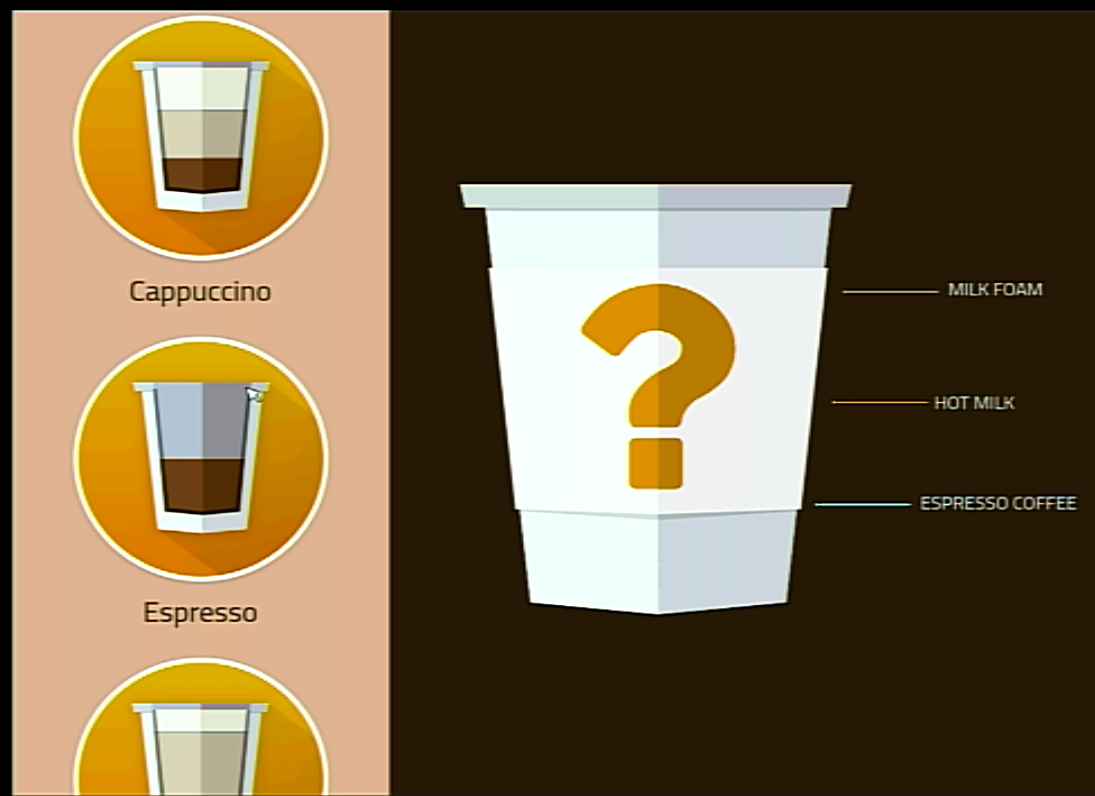
\includegraphics[width=5cm]{assets/Screenshot_Coffee_QT6.4.2.png} &
		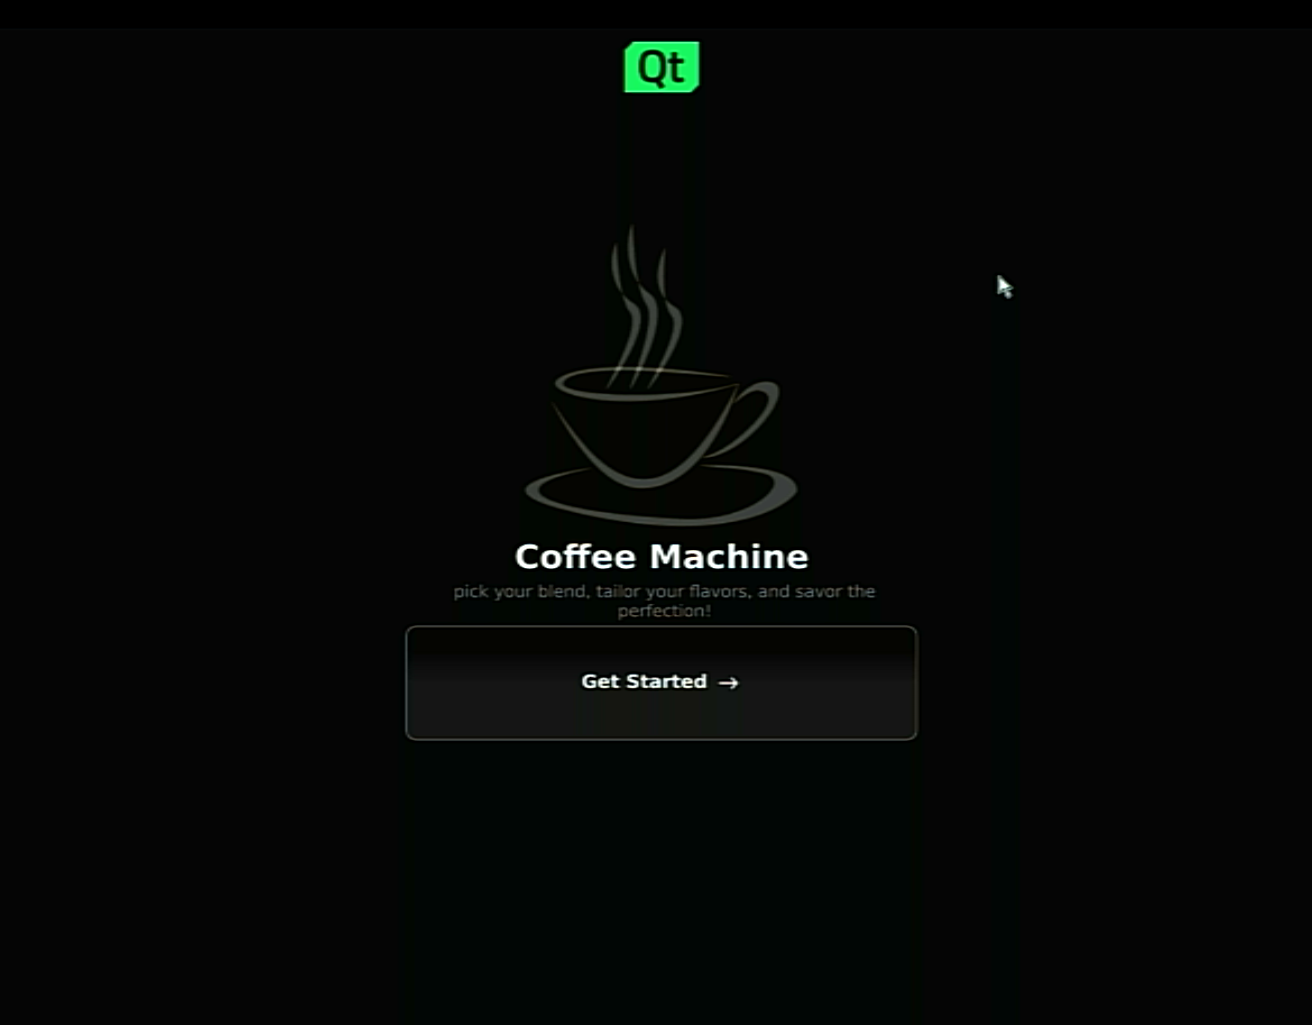
\includegraphics[width=5cm]{assets/Screenshot_Coffee_QT6.6.2.png} \\
	\end{tabular}
	% In the implementation, we will use QT 6.6.2, for Yocto, because it's the latest
	% version and a Yocto metalayer is available.
	% For elbe, we will use QT 6.4.2, because it's the version provided by Debian Bookworm.
	% In the Github repo, you also find instrutions how to cross-compile QT 6.6.2 for
	% the Rasbperry Pi 4, but this is an bad idea because of the maintenance impact.
	% A better approach would be, if QT 6.6.2 is really mandatory, to use it from
	% Debian experimental.
\end{frame}

\subsection{Coffee machine with Yocto}

\begin{frame}{How to realize this project with Yocto?}
	\begin{block}{How to do?}
		How to implement the coffee machine project with Yocto?
	\end{block}
	% The next slides will show step by step how to implement the
	% coffee machine with Yocto.
\end{frame}

\subsection{Coffee machine with Elbe}

\begin{frame}{How to realize this project with Elbe?}
	\begin{block}{How to do?}
		How to implement the coffee machine project with Elbe?
	\end{block}
	% The next slides will show step by step how to implement the
	% coffee machine with Yocto.
\end{frame}

\begin{frame}{How to realize this project with Elbe?}
	\begin{block}{Using the Debian Bookworm QT packages}
		How to implement the coffee machine project with Elbe using the QT 6.4.2 packages provided by Debian Bookworm?
	\end{block}

	You can find the code for this example on
	\href{https://github.com/tomirgang/eh21_maintainable_linux/tree/main/examples/elbe_advanced}{Github}.
	% You can find a more detailed description on Github.
\end{frame}


\begin{frame}{Step 1: Ensure we can build the app}
	First we should make sure we can build the app:
	\begin{itemize}
		\item Install the needed build dependencies:\\
			\emph{sudo apt install qt6-base-dev qt6-declarative-dev}
		\item Get the source code of the example app
		\item Create a build folder and build the app:
		\begin{itemize}
			\item cmake \emph{path-to/coffee}
			\item make
		\end{itemize}
	\end{itemize}
	This should give you a \emph{coffee} binary which you can run.
	% A good first step is to build the app on a host machine running
	% the same distribution. This allows more easy development and testing,
	% and helps to find out the needed build- and runtime-dependencies.
	% For Debian Bookworm, we need the packages qt6-base-dev and qt6-declarative-dev.
	% Then building the app with cmake is straight forward.
\end{frame}

\begin{frame}{Step 2: Package the app - Debian metadata}
	Next we should create a Debian package for our app.\\
	To do this, we need to generate Debian metadata for the app:
	\begin{itemize}
		\item Install the needed tools:\\
		\emph{sudo apt install dh-make pbuilder debootstrap devscripts}
		\item Set the needed Debian maintainer environment variables:
		\begin{itemize}
			\item \emph{export DEBFULLNAME="Thomas Irgang"}
			\item \emph{export DEBEMAIL="thomas@irgang.eu"}
		\end{itemize}
		\item Rename the app folder using the pattern: \emph{app name}-\emph{app version}
		\item Generate the Debian metadata:
		\begin{itemize}
			\item Inside the app folder, run:
			\item \emph{dh\_make -n -s --yes}
		\end{itemize}
	\end{itemize}
	This will generate a \emph{debian} sub-folder containing lot's of prepared package metadata.
	% The best was to add our app to the image, and to make the app resuable, is to
	% package it. For packkaging the app we need dh-make, pbuilder, debootstrap, and
	% devscripts.
	% Creating a package for submitting it to Debian is some effot, but packaging
	% the app just for us is quite simple. The Debian tooling expects the environment
	% variables DEBFULLNAME and DEBEMAIL, wich describe the maintianer. You can set it
	% using export, or add the lines to your shellrc file.
	% dh_make expexts the sources to be in a folder with the naming pattern
	% app-name - app-verison. When this is prepared, we can generate dh_make in
	% this folder.
\end{frame}

\begin{frame}{Step 3: Package the app - fine-tune metadata}
	Now we need to fine-tune the generated metadata:
	\begin{itemize}
		\item Add the build dependencies:
		\begin{itemize}
			\item \emph{qt6-base-dev}
			\item \emph{qt6-declarative-dev}
		\end{itemize}
		\item During the package build, shared library dependencies will be filled automatically by \emph{shlibs}, but we need to add manually the dynamic loaded libraries:
		\begin{itemize}
			\item \emph{qml6-module-qtquick}
			\item \emph{qml6-module-qtquick-controls}
			\item \emph{qml6-module-qtquick-layouts}
			\item \emph{qml6-module-qtquick-templates}
			\item \emph{qml6-module-qtquick-window}
			\item \emph{qml6-module-qtqml-workerscript}
		\end{itemize}
	\end{itemize}
	% This will give us Debian package metadata, including man-page templates and
	% lot's of other stuff, we can ignore if we don't want to publish the app.
	% There are only two mandatory changes we need to do:
	% We need to add the build dependnecies,
	% and we need to add the dynamic runtime dependencies which the Debian tooling
	% cannot derive.
\end{frame}

\begin{frame}{Step 4: Package the app - configure pbuilder}
	Our image is based on Debian Bookwork. Configure pbuilder:
	\begin{itemize}
		\item Create \emph{.pbuilderrc}:
	\end{itemize}
	
	\small{\emph{echo "DISTRIBUTION=bookworm" $>>$ ~/.pbuilderrc} \\
	\emph{echo "MIRRORSITE=http://ftp.de.debian.org/debian" $>>$ ~/.pbuilderrc}}
	
	\begin{itemize}
		\item For cross-compilation support, we need to enable the apt dependency resolution:
	\end{itemize}
	\small{\emph{echo 'PBUILDERSATISFYDEPENDSCMD="/usr/lib/pbuilder/pbuilder-satisfydepends-apt"' $>>$ ~/.pbuilderrc}}
	% For building the multi-arch package, we can use pbuilder.
	% Multi-arch is the Debian way of cross-compiling.
	% We could use lots of commandline arguments, but the better way is to create
	% a pbuilderrc file, which tells pbuilder about our target distribution and
	% the tooling for dependency checking.
\end{frame}

\begin{frame}{Step 5: Package the app - build the package}
	Now we can build the app:
	\begin{itemize}
		\item Run \emph{pdebuild} in the folder containing the coffee app: \\ \emph{pdebuild -- --host-arch arm64}
	\end{itemize}
	This will generate a \emph{coffee\_6.4.2\_arm64.deb} in \emph{/var/cache/pbuilder/result}.
	% Now we can build any Debian source package for our target platform.
	% To build our coffee app package, run pdebuild -- --host-arch arm64
	% in the folder containing the app sources.
	% This will create a Debian binary package for arm64 containing your app in
	% /var/cache/pbuilder/result.
\end{frame}

\begin{frame}{Step 6: Auto-start the app}
	Automatically run the app on system startup:
	\begin{itemize}
		\item Create a systemd unit file to run the binary.
		\href{https://github.com/tomirgang/eh21_maintainable_linux/blob/main/examples/elbe_advanced/image/rpi-image/overlays/systemd/etc/systemd/system/coffee.service}{Github}
		\item Enable the new service using a \emph{finetuning} command:
		\begin{itemize}
			\item \emph{$<$command variant="app"$>$systemctl enable coffee$<$/command$>$}
		\end{itemize}
		\item Disable the getty on the HDMI tty:
		\begin{itemize}
			\item \emph{$<$command variant="app"$>$systemctl mask getty@tty1$<$/command$>$}
			\item \emph{$<$command variant="app"$>$systemctl disable getty@tty1$<$/command$>$}
		\end{itemize}
	\end{itemize}
	% For the project, we want to automatically run the app on system startup
	% without any user interaction. We can do this using systemd and some elbe
	% finetuning commands.
	% The git repo contains a very small systemd unit file to run the app.
	% When this is added to the image, using a root filesystem overlay, we can
	% run the app by enabling the service.
	% We also need to disable the getty running on the HDMI tty, to aviod
	% over-drawing our app with a login shell.
	% For "production", we should add the systemd unit file to the Debian package,
	% and use the post-install script to enable the service. 
\end{frame}

\begin{frame}{Step 7: Install the app}
	\begin{itemize}
		\item Add app to image description: \emph{$<$pkg variant="app"$>$coffee$<$/pkg$>$}
		\item Build image with app:
		\small{\begin{itemize}
				\item \emph{elbe control create\_project $>$ my.prj}
				\item \emph{export PRJ=\$(cat my.prj)}
				\item \emph{elbe preprocess --variant app rpi-image/aarch64\_rpi4.xml}
				\item \emph{elbe control set\_xml \$PRJ preprocess.xml}
				\item \emph{elbe prjrepo upload\_pkg \$PRJ /var/cache/pbuilder/result/coffee\_6.4.2\_arm64.deb}
				\item \emph{elbe control build \$PRJ}
				\item wait for build finishing and download results.
		\end{itemize}}
	\end{itemize}
	% Next we can build your image including the app. To allow elbe to install the
	% app, we need to make it available to the build. On way would be to setup our
	% own local apt repository, but since we have only one package, uploading it
	% to the elbe project is more easy.
	% The elbe control commands allow quite low level control over the build process.
	% To build the image, we first create the elbe project, prepare our image descripiton,
	% make our app package available in the project, build the image and
	% download the image.
\end{frame}

\section{The End}

\begin{frame}{The End}
	\begin{block}{Any questions?}
		We hope you enjoyed the talk.
		Your questions are now welcome!
	\end{block}
\end{frame}

% Backup slides

\section{How to build a Raspberry Pi image?}


\begin{frame}{Yocto: Raspberry Pi image}
	\begin{itemize}
		\item Source: \href{https://git.yoctoproject.org/poky}{poky}, \href{https://git.yoctoproject.org/meta-raspberrypi/}{bsp}
		\item based on Poky
		\item Steps:
		\begin{itemize}
			\item install kas: pip3 install kas
			\item get kas.yml
			\item run kas build
			\item copy image to SD card
		\end{itemize}
		\item more details on \href{https://github.com/tomirgang/eh21_maintainable_linux/tree/main/examples/first_build_rpi4/yocto}{Github}
	\end{itemize}
\end{frame}


\begin{frame}{Buildroot: Raspberry Pi image}
	\begin{itemize}
		\item Source: \href{https://gitlab.com/buildroot.org/buildroot/}{GitLab}
		\item Steps:
		\begin{itemize}
			\item install \href{https://buildroot.org/downloads/manual/manual.html\#requirement}{dependencies}
			\item make raspberrypi4\_64\_defconfig
			\item make
			\item copy image to SD card
		\end{itemize}
		\item more details on \href{https://github.com/tomirgang/eh21_maintainable_linux/tree/main/examples/first_build_rpi4/buildroot}{Github}
	\end{itemize}
\end{frame}

\begin{frame}{Kiwi-ng: Raspberry Pi image}
	\begin{itemize}
		\item Source: \href{https://github.com/OSInside/kiwi-descriptions/tree/main/ubuntu/aarch64/ubuntu-jammy-rpi}{Github}
		\item based on Ubuntu Jammy
		\item Steps:
		\begin{itemize}
			\item install \url{https://pypi.org/project/kiwi/}
			\item install \url{https://pypi.org/project/kiwi-boxed-plugin/}
			\item get image description
			\item run image build
			\item copy image to SD card
		\end{itemize}
		\item more details on \href{https://github.com/tomirgang/eh21_maintainable_linux/tree/main/examples/first_build_rpi4/kiwi-ng}{Github}
	\end{itemize}
\end{frame}


\begin{frame}{Debos: Raspberry Pi image}
	\begin{itemize}
		\item Source: \href{https://github.com/go-debos/debos-recipes/tree/main/rpi64}{Github}
		\item based on Debian Bullseye
		\item Steps:
		\begin{itemize}
			\item Debian: install debos packages
			\item run image build
			\item copy image to SD card
		\end{itemize}
		\item more details on \href{https://github.com/tomirgang/eh21_maintainable_linux/tree/main/examples/first_build_rpi4/debos}{Github}
	\end{itemize}
\end{frame}


\begin{frame}{Elbe: Raspberry Pi image}
	\begin{itemize}
		\item Based on \href{https://github.com/Linutronix/elbe/blob/master/examples/arm64-qemu-virt.xml}{example arm64-qemu-virt}
		\item Steps:
		\begin{itemize}
			\item Debian: install elbe package
			\item prepare the initvm
			\item run the image build
			\item copy image to SD card
		\end{itemize}
		\item more details on \href{https://github.com/tomirgang/eh21_maintainable_linux/tree/main/examples/first_build_rpi4/elbe}{Github}
	\end{itemize}
\end{frame}


\end{document}
